\chapter{Аналитическая часть}

\section{Иерархическая кластеризация}

Среди алгоритмов иерархической кластеризации выделяются два основных типа.
\begin{enumerate}[label*=\arabic*.]
	\item \textbf{Нисходящая кластеризация (divisive)}: Работает
	по принципу <<сверху-вниз>>: в начале, все объекты
	принадлежат одному кластеру. В ходе
	итеративного процесса крупные кластеры
	разделяются на более мелкие. Такие задачи
	называются задачами таксономии. При этом,
	получается дерево кластеров (дендрограмма).
	\item  \textbf{Восходящая кластеризация (agglomerative)}:
	Изначально каждый элемент множества является
	отдельным кластером. Процесс образования
	новых кластеров заключается в объединение
	некоторых кластеров в один на основе заданного
	расстояния. В итоге итеративного объединения
	получаем дерево, которое сходится к одному
	кластеру.
\end{enumerate}

На рисунке \ref{img:algo} представлена иллюстрация работы иерархической кластеризации.
\begin{figure}
	\begin{center}
		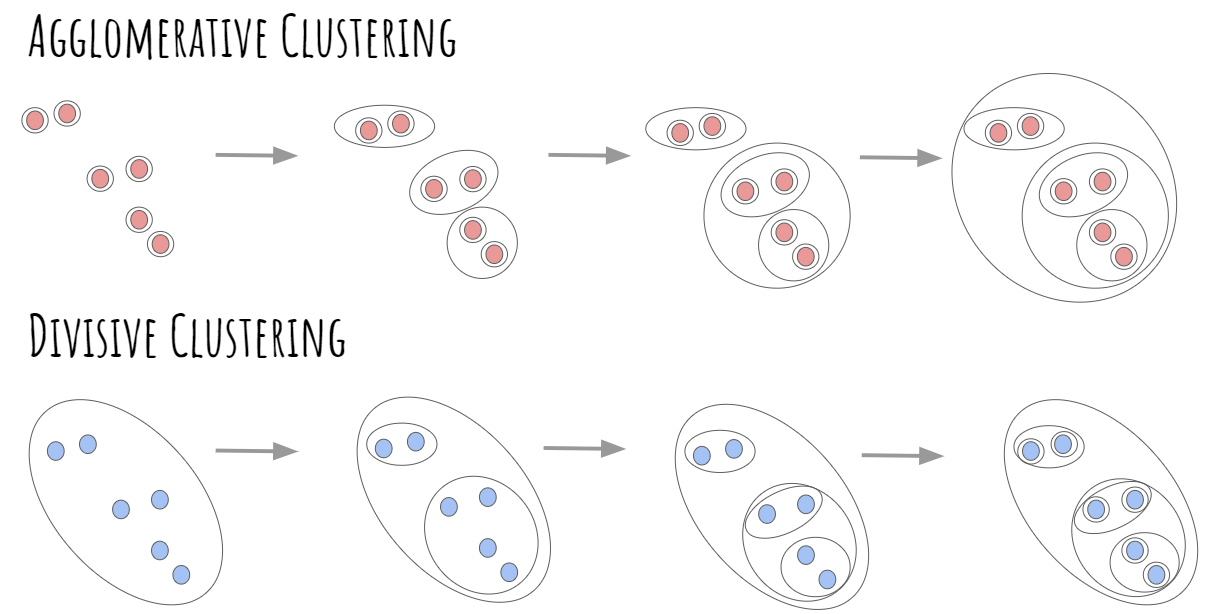
\includegraphics[width=\textwidth]{images/algo.png}
	\end{center}
	\caption{Иерархическая кластеризация}
	\label{img:algo}
\end{figure}

\FloatBarrier



\section{Алгоритм HDBSCAN}

Density-based spatial clustering of applications with noise (DBSCAN) ---
основанная на плотности пространственная кластеризация для
приложений с шумами.

Если дан набор точек в некотором пространстве, алгоритм группирует
вместе точки, которые тесно расположены (точки со многими близкими
соседями), помечая как выбросы точки, которые находятся одиноко в
областях с малой плотностью (ближайшие соседи которых лежат далеко).
DBSCAN развивает идею кластеризации с помощью выделения связных
компонент.

Алгоритм HDBSCAN расширяет DBSCAN за счёт автоматического определения оптимальных параметров кластеризации (например, не требует ручного выбора радиуса $\varepsilon$), что особенно полезно для данных с переменной плотностью кластеров. Кроме того, HDBSCAN строит иерархическую структуру кластеров, что позволяет выделять устойчивые группы даже при сложном распределении данных, и эффективно обрабатывает выбросы. Алгоритм также демонстрирует инвариантность к масштабу данных, что упрощает его применение без предварительной нормализации исходных данных.


\clearpage
